\chapter{Task 35}

\resp{Asal Kermaniha}

\subsection{Introduction}
We consider two articles discussing two different but related models of collective behavior on networks. The first article studies the interplay between social and strategic imitation, while the second studies the coevolution of synchronization and cooperation in costly networked interactions.
\noindent
In both models, we construct two networks \(G=(V,E)\), where the nodes represent agents and the edges represent interactions between them. We tried to reproduce the main results of both articles.

\subsection{First Model}\cite{vilone2012}

\noindent
Each agent is allowed to have two possible strategies:
\[
s_i \in \{A, B\}
\]
\noindent
The payoff for each agent is computed as follows:
\[
\Pi_i = \sum_{j \in N(i)} \delta(s_i, s_j)
\]
\noindent
In the first step, the strategies are assigned randomly. Then, we have two different update rules:

\subsubsection{Unconditional imitation}

Each node finds the neighbor with the highest payoff, provided that this payoff is larger than its own payoff.

\subsubsection{Voter model}

The agent copies the strategy of a randomly selected neighbor.

\noindent
With probability \(q\), the agent follows the voter model; otherwise, it follows unconditional imitation.
\newpage

\subsection{Second Model}\cite{antonioni2017}

\noindent
In the second model, each node has both a phase \(\theta_i\), representing a Kuramoto oscillator, and a strategy, cooperator, or defector. In the first step, both the strategies and the phases are randomly assigned.

\noindent
The payoff for each node is calculated as follows:
\[
\Pi_i =
r_i
-
\alpha
\frac{\left|\Delta \theta_i\right|}{2\pi}
\]

\noindent
The first term is the benefit of each node, which indicates local synchronization:
\[
r_i = \frac{1}{k_i}
\left|
\sum_{j \in N_i}
e^{i\theta_j}
\right|
\]

\noindent
The second term is a penalty term that indicates the cost of synchronization when the node has chosen the cooperative strategy.

\noindent
Each node's strategy is updated according to the Fermi rule:
\[
P(s_i \leftarrow s_j)
=
\frac{1}
{1+\exp\!\left[-\beta\left(\Pi_j-\Pi_i\right)\right]}
\]
\subsection{Analytics and results}
Both articles investigate the effect of model hyper parameters on the convergence dynamics of the network.
with the first model, the hyperparameter is \(q\) which is the probability of each agent to follow the voter model update strategy.

\noindent
The variation of \(tau\) as a function of q is observed for homogeneous(ER) and scale free(BA) networks.
The characteristic ordering time $\tau$ is defined as

\[
\tau = \min \left\{ t : n_A(t) < 10^{-2} \right\},
\]

\noindent
IE., the Monte Carlo time required for the density of active links $n_A(t)$ to decrease below $10^{-2}$.(Figure 1.2)

\noindent
A logarithmic graph has also been reconstructed for the ER network, showing the time evolution of the active link density in different Monte Carlo steps for various values of $q$.(Figure 1.1).The figure demonstrates a dramatic decrease in the fraction of agents adopting the strategy $A$, $n_A(t)$, for $q=0.15$ and $q=0.35$ compared to the lower noise level $q=0.05$.

\noindent
In the second article, instead, the hyperparameter is the coupling strength $\lambda$, and the model is also implemented on a RGG (Random Geometric Graph).the observed parameter is Local Neighborhood Synchronization: \[
\langle r_L \rangle_k
\]Figure 1.3 demonstrates the relation between these two parameters, revealing a resonance-like behavior in which local synchronization reaches a maximum at intermediate coupling strengths before decaying at higher values of $\lambda$.


\begin{figure}[ht]
    \centering
    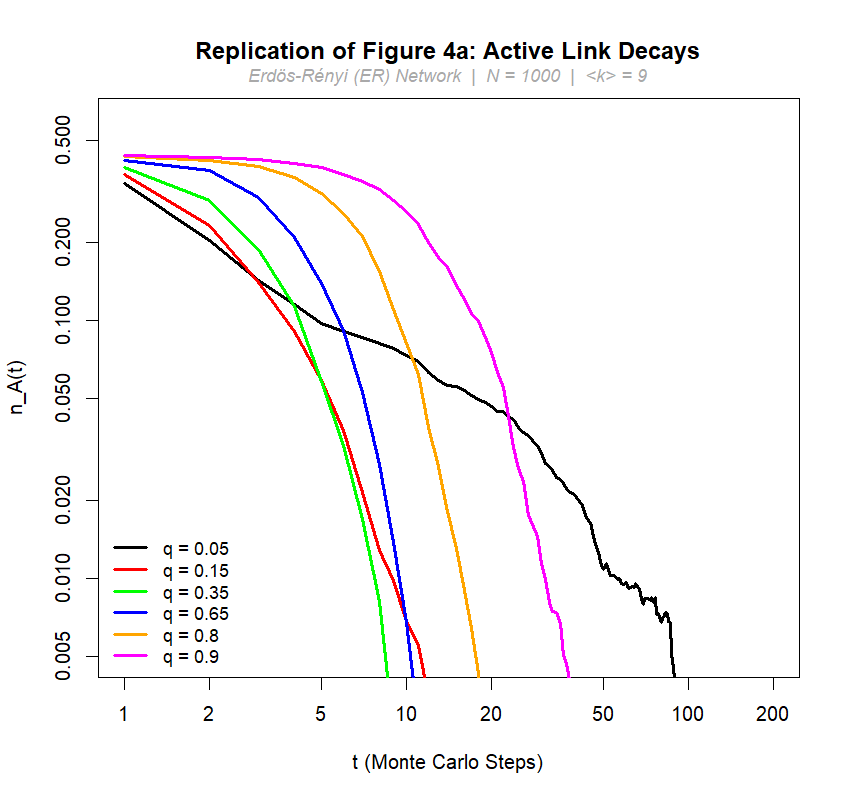
\includegraphics[width=0.5\textwidth]{images/theorical_project_plots/active_link_decay_fig4a.png}
    \caption{Synchronization level as a function of coupling strength.}
    \label{fig:sync}
\end{figure}

\noindent
\begin{figure}[H]
\centering

\begin{minipage}{0.48\textwidth}
\centering
\textbf{(a)}\\[1mm]
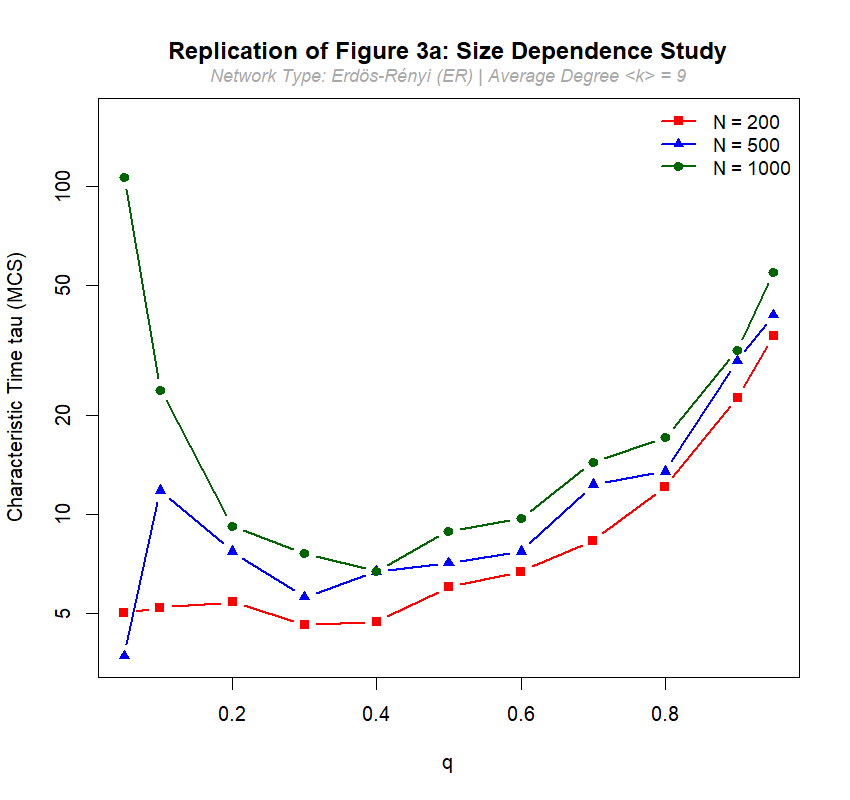
\includegraphics[width=\linewidth]{images/theorical_project_plots/u_shape_multi_N_ER.png}
\end{minipage}
\hfill
\begin{minipage}{0.48\textwidth}
\centering
\textbf{(b)}\\[1mm]
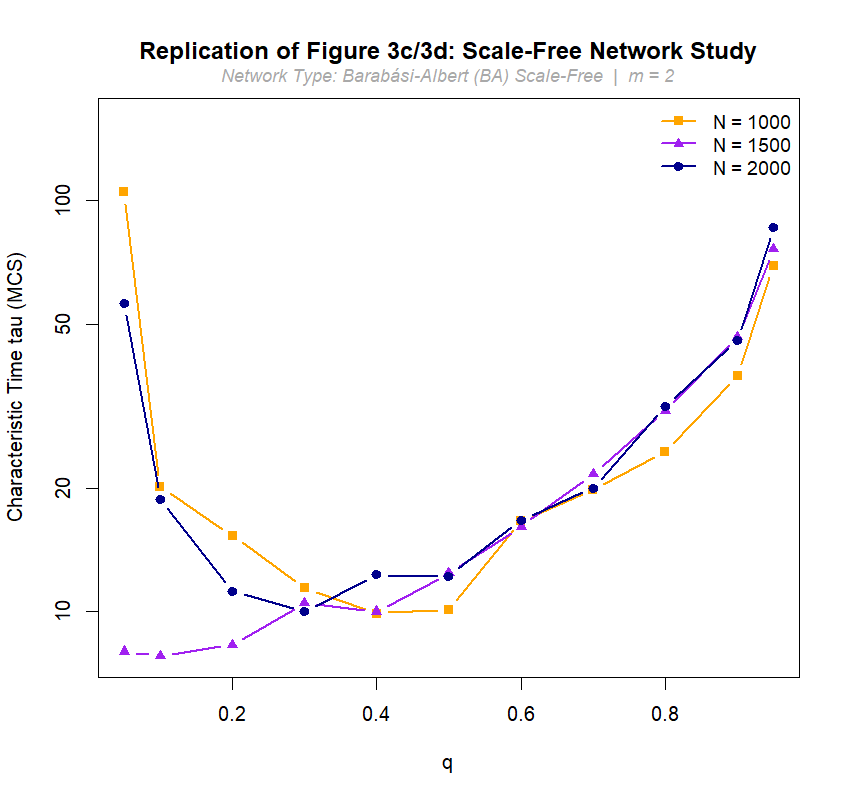
\includegraphics[width=\linewidth]{images/theorical_project_plots/u_shape_multi_N.png}
\end{minipage}

\caption{for both networks In small sizes, the limited size prevents achieving to the article's results. because small stochastic fluctuations quickly drive the system to early consensus, once the network is big enough, we can see the expected U shape for both cases indicating the existence of a clear minimum in this intermediate range for (a) ER network and (b) Scale-free network}
\label{fig:comparison}
\end{figure}
\noindent
\begin{figure}[H]
    \centering
    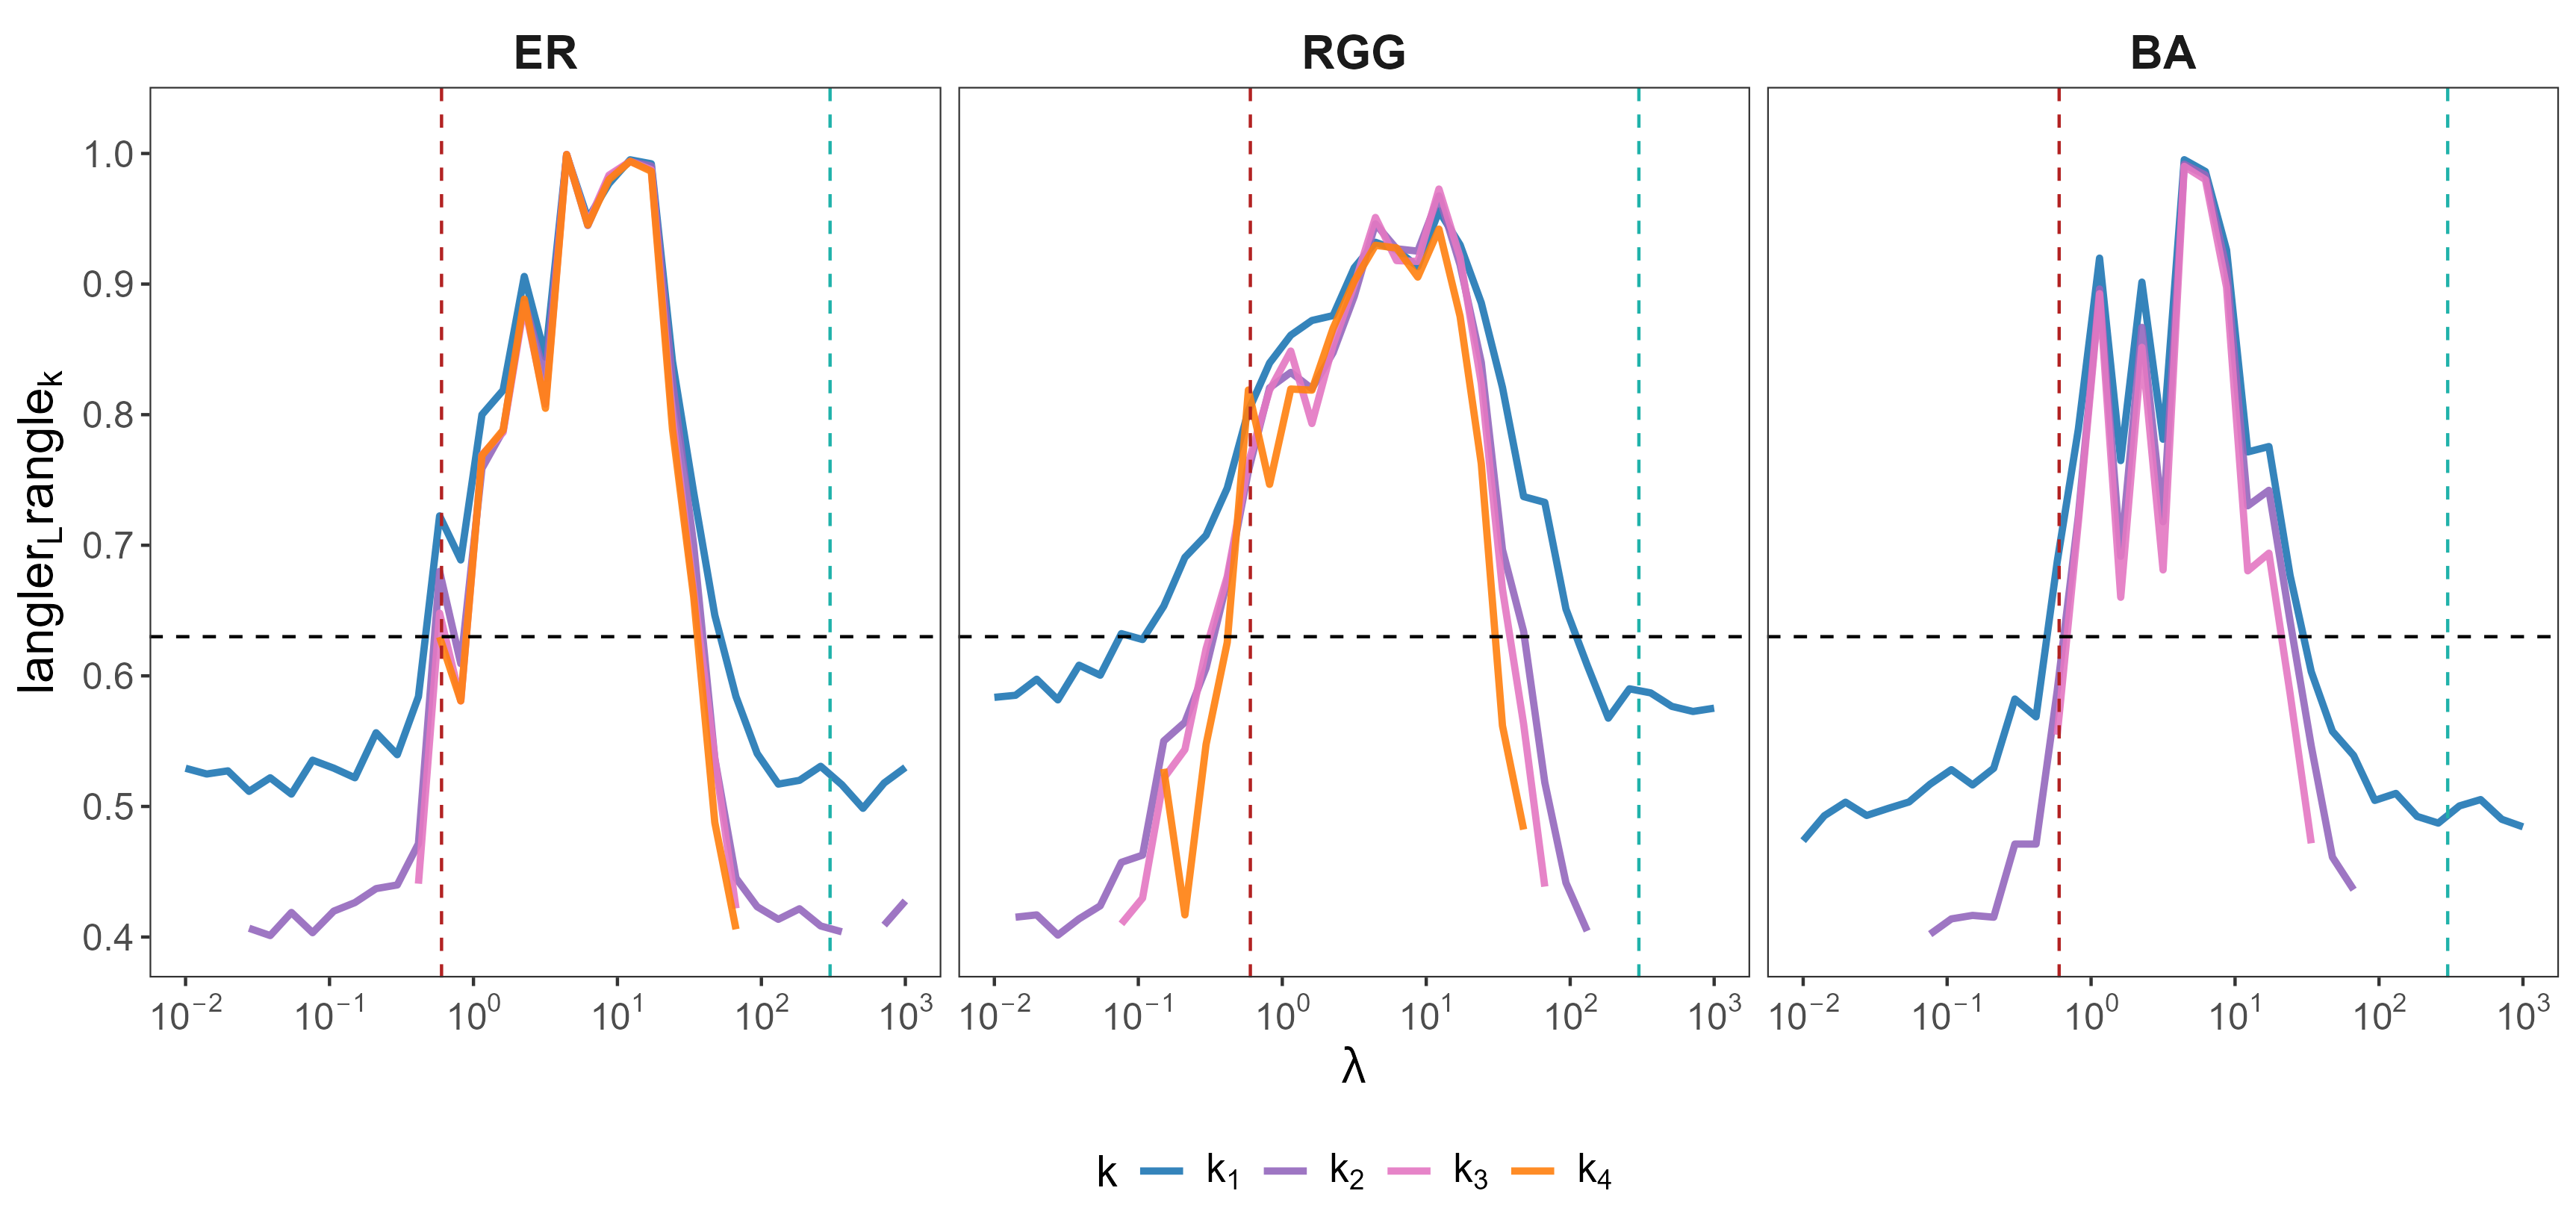
\includegraphics[width=0.8\textwidth]{images/theorical_project_plots/PRL_replication_plot.png}
    \caption{Synchronization level as a function of coupling strength. All of the networks have same amount of mean degree=6. the different colors represent the four distinct degree classes ($k_1$ to $k_4$), }
    \label{fig:sync}
\end{figure}

\noindent
*For the second model's implementation, ChatGPT (OpenAI) was used to assist in optimizing the implementation of the code in response to computational constraints, including improvements related to execution time, memory usage, and debugging of the analysis pipeline.
\subsection{conclusion}
Implementing both models, we could understand that in dynamic networks investigated, ultimate order and consensus are never reached through extremes; rather, everything hinges upon a universal, delicate trade-off.

